%%
%% This is file `sample-sigconf.tex',
%% generated with the docstrip utility.
%%
%% The original source files were:
%%
%% samples.dtx  (with options: `sigconf')
%% 
%% IMPORTANT NOTICE:
%% 
%% For the copyright see the source file.
%% 
%% Any modified versions of this file must be renamed
%% with new filenames distinct from sample-sigconf.tex.
%% 
%% For distribution of the original source see the terms
%% for copying and modification in the file samples.dtx.
%% 
%% This generated file may be distributed as long as the
%% original source files, as listed above, are part of the
%% same distribution. (The sources need not necessarily be
%% in the same archive or directory.)
%%
%%
%% Commands for TeXCount
%TC:macro \cite [option:text,text]
%TC:macro \citep [option:text,text]
%TC:macro \citet [option:text,text]
%TC:envir table 0 1
%TC:envir table* 0 1
%TC:envir tabular [ignore] word
%TC:envir displaymath 0 word
%TC:envir math 0 word
%TC:envir comment 0 0
%%
%%
%% The first command in your LaTeX source must be the \documentclass
%% command.
%%
%% For submission and review of your manuscript please change the
%% command to \documentclass[manuscript, screen, review]{acmart}.
%%
%% When submitting camera ready or to TAPS, please change the command
%% to \documentclass[sigconf]{acmart} or whichever template is required
%% for your publication.
%%
%%

\PassOptionsToPackage{table}{xcolor}
\documentclass[sigconf]{acmart}


%%
%% \BibTeX command to typeset BibTeX logo in the docs
\AtBeginDocument{%
  \providecommand\BibTeX{{%
    Bib\TeX}}}

%% Rights management information.  This information is sent to you
%% when you complete the rights form.  These commands have SAMPLE
%% values in them; it is your responsibility as an author to replace
%% the commands and values with those provided to you when you
%% complete the rights form.
\setcopyright{acmcopyright}
\copyrightyear{2018}
\acmYear{2018}
\acmDOI{XXXXXXX.XXXXXXX}

%% These commands are for a PROCEEDINGS abstract or paper.
\acmConference[Conference acronym 'XX]{Make sure to enter the correct
  conference title from your rights confirmation emai}{June 03--05,
  2018}{Woodstock, NY}
%%
%%  Uncomment \acmBooktitle if the title of the proceedings is different
%%  from ``Proceedings of ...''!
%%
%%\acmBooktitle{Woodstock '18: ACM Symposium on Neural Gaze Detection,
%%  June 03--05, 2018, Woodstock, NY}
\acmPrice{15.00}
\acmISBN{978-1-4503-XXXX-X/18/06}



%%
%% Submission ID.
%% Use this when submitting an article to a sponsored event. You'll
%% receive a unique submission ID from the organizers
%% of the event, and this ID should be used as the parameter to this command.
%%\acmSubmissionID{123-A56-BU3}

%%
%% For managing citations, it is recommended to use bibliography
%% files in BibTeX format.
%%
%% You can then either use BibTeX with the ACM-Reference-Format style,
%% or BibLaTeX with the acmnumeric or acmauthoryear sytles, that include
%% support for advanced citation of software artefact from the
%% biblatex-software package, also separately available on CTAN.
%%
%% Look at the sample-*-biblatex.tex files for templates showcasing
%% the biblatex styles.
%%

%%
%% The majority of ACM publications use numbered citations and
%% references.  The command \citestyle{authoryear} switches to the
%% "author year" style.
%%
%% If you are preparing content for an event
%% sponsored by ACM SIGGRAPH, you must use the "author year" style of
%% citations and references.
%% Uncommenting
%% the next command will enable that style.
%%\citestyle{acmauthoryear}

\usepackage{makecell}
\usepackage{multirow}

%%
%% end of the preamble, start of the body of the document source.
\begin{document}

%%
%% The "title" command has an optional parameter,
%% allowing the author to define a "short title" to be used in page headers.

% \usepackage{color, colortbl}
\definecolor{nsig}{rgb}{1,0.7,0.7}
\definecolor{sig}{rgb}{0.7,1,0.7}

\title{Revisiting Intention Estimation: \\Defining Unrealized and Realized Social Intentions In-the-wild}
%reframining intention estimation in terms of realised and unrealised intentions
%%
%% The "author" command and its associated commands are used to define
%% the authors and their affiliations.
%% Of note is the shared affiliation of the first two authors, and the
%% "authornote" and "authornotemark" commands
%% used to denote shared contribution to the research.
% \author{Hayley Hung, Litian Li,  Jord Molhoek, and  Jing Zhou}

% \email{h.hung@tudelft.nl}

% % \authornotemark[1]
% % \email{webmaster@marysville-ohio.com}
% \affiliation{%
%   \institution{Delft University of Technology}
%   \country{The Netherlands}
% }
\author{anon}
\email{anon}

\affiliation{\institution{anon}
\country{anon}}


% \author{Lars Th{\o}rv{\"a}ld}
% \affiliation{%
%   \institution{The Th{\o}rv{\"a}ld Group}
%   \streetaddress{1 Th{\o}rv{\"a}ld Circle}
%   \city{Hekla}
%   \country{Iceland}}
% \email{larst@affiliation.org}

% \author{Valerie B\'eranger}
% \affiliation{%
%   \institution{Inria Paris-Rocquencourt}
%   \city{Rocquencourt}
%   \country{France}
% }

% \author{Aparna Patel}
% \affiliation{%
%  \institution{Rajiv Gandhi University}
%  \streetaddress{Rono-Hills}
%  \city{Doimukh}
%  \state{Arunachal Pradesh}
%  \country{India}}

% \author{Huifen Chan}
% \affiliation{%
%   \institution{Tsinghua University}
%   \streetaddress{30 Shuangqing Rd}
%   \city{Haidian Qu}
%   \state{Beijing Shi}
%   \country{China}}

% \author{Charles Palmer}
% \affiliation{%
%   \institution{Palmer Research Laboratories}
%   \streetaddress{8600 Datapoint Drive}
%   \city{San Antonio}
%   \state{Texas}
%   \country{USA}
%   \postcode{78229}}
% \email{cpalmer@prl.com}

% \author{John Smith}
% \affiliation{%
%   \institution{The Th{\o}rv{\"a}ld Group}
%   \streetaddress{1 Th{\o}rv{\"a}ld Circle}
%   \city{Hekla}
%   \country{Iceland}}
% \email{jsmith@affiliation.org}

% \author{Julius P. Kumquat}
% \affiliation{%
%   \institution{The Kumquat Consortium}
%   \city{New York}
%   \country{USA}}
% \email{jpkumquat@consortium.net}

%%
%% By default, the full list of authors will be used in the page
%% headers. Often, this list is too long, and will overlap
%% other information printed in the page headers. This command allows
%% the author to define a more concise list
%% of authors' names for this purpose.
\renewcommand{\shortauthors}{anon et al.}

%%
%% The abstract is a short summary of the work to be presented in the
%% article.
\begin{abstract}
 The future of socially intelligent systems depends on developing abilities to anticipate and empathize with users. Whilst great strides have been made on developing systems for future behavior forecasting that sometimes also claim to do intention estimation, we argue that the predominant state-of-the-art treatment of these problems leads to a significant misunderstanding about this topic. This paper revisits this topic, describing the "intention by outcome" problem and how it severely limits a deeper understanding of the nature of the intention estimation problem. Through a case study on estimating unrealized intentions to speak in-the-wild, we highlight open challenges of this largely unexplored topic.
\end{abstract}

%%
%% The code below is generated by the tool at http://dl.acm.org/ccs.cfm.
%% Please copy and paste the code instead of the example below.
%%
% \begin{CCSXML}
% <ccs2012>
%  <concept>
%   <concept_id>10010520.10010553.10010562</concept_id>
%   <concept_desc>Computer systems organization~Embedded systems</concept_desc>
%   <concept_significance>500</concept_significance>
%  </concept>
%  <concept>
%   <concept_id>10010520.10010575.10010755</concept_id>
%   <concept_desc>Computer systems organization~Redundancy</concept_desc>
%   <concept_significance>300</concept_significance>
%  </concept>
%  <concept>
%   <concept_id>10010520.10010553.10010554</concept_id>
%   <concept_desc>Computer systems organization~Robotics</concept_desc>
%   <concept_significance>100</concept_significance>
%  </concept>
%  <concept>
%   <concept_id>10003033.10003083.10003095</concept_id>
%   <concept_desc>Networks~Network reliability</concept_desc>
%   <concept_significance>100</concept_significance>
%  </concept>
% </ccs2012>
% \end{CCSXML}

% \ccsdesc[500]{Computer systems organization~Embedded systems}
% \ccsdesc[300]{Computer systems organization~Redundancy}
% \ccsdesc{Computer systems organization~Robotics}
% \ccsdesc[100]{Networks~Network reliability}

% \begin{CCSXML}
% <ccs2012>
%    <concept>
%        <concept_id>10003120.10003138.10003139.10010904</concept_id>
%        <concept_desc>Human-centered computing~Ubiquitous computing</concept_desc>
%        <concept_significance>500</concept_significance>
%        </concept>
   
%  </ccs2012>
% \end{CCSXML}

% \ccsdesc[500]{Human-centered computing~Ubiquitous computing}
%%
%% Keywords. The author(s) should pick words that accurately describe
%% the work being presented. Separate the keywords with commas.
\keywords{intention estimation, in the wild, speaking}
%% A "teaser" image appears between the author and affiliation
%% information and the body of the document, and typically spans the
%% page.
\begin{teaserfigure}
  \begin{tabular}{cc}
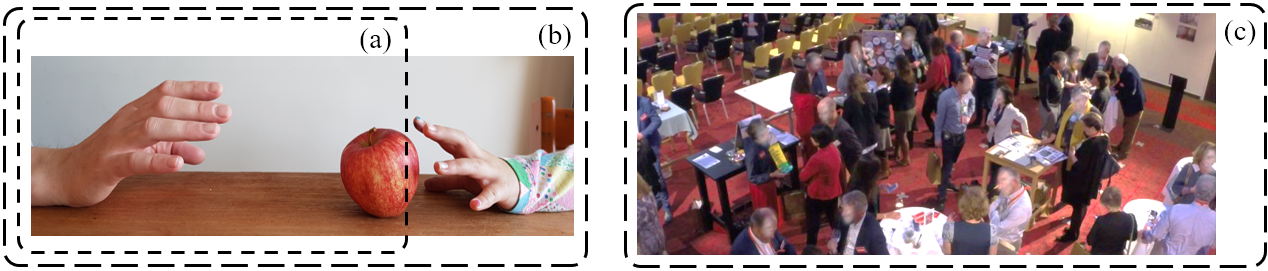
\includegraphics[width=0.66\textwidth]{samples/Teaser.png} & 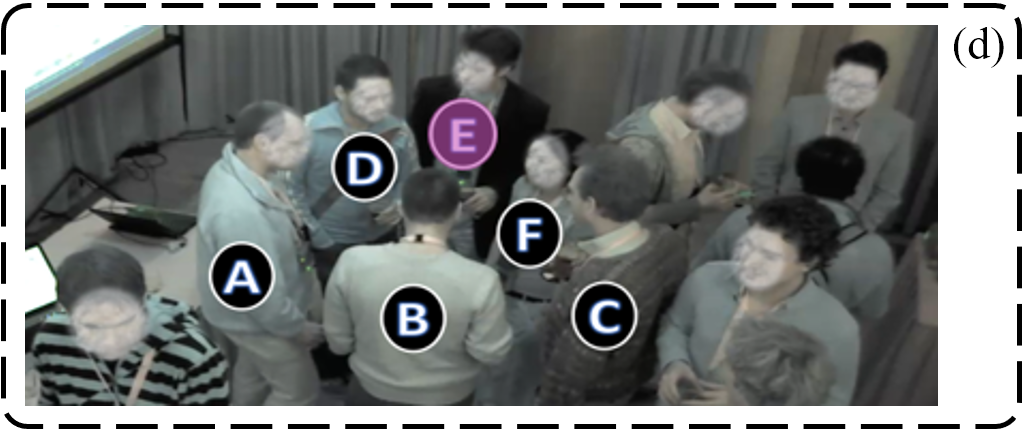
\includegraphics[width=0.33\textwidth]{samples/AnnotatedSocialStill.png}
  \end{tabular}
  \caption{Illustration of the intention by outcome problem. (a): Common setups involve an individual grabbing objects with gaze and posture. (b): When 2 or more people operate with competing goals, realized as well as unrealized intentions can occur. (c): Example of a crowded in-the-wild setting where people operate with hidden individual goals; coordinating to speak, leave, and join conversations emerge simultaneously with (un)realized intentions. (d) Does E intend to speak to D?}
  \label{fig:teaser}
\end{teaserfigure}

\received{20 February 2007}
\received[revised]{12 March 2009}
\received[accepted]{5 June 2009}

%%
%% This command processes the author and affiliation and title
%% information and builds the first part of the formatted document.
\maketitle

\section{Introduction}
Effective multi-modal interaction relies on the ability to anticipate and empathize with humans. As a result, many researchers have investigated the problem of intention estimation \cite{Huang2015,Nie2021,CAO20171,objectpicking2021} and behavior forecasting \cite{ramansocproc2021,humantrajpredict2020}. One of the more popular approaches to designing and evaluating the effectiveness of intent prediction systems is using object picking tasks \cite{Huang2015,objectpicking2021}, which is very relevant in situations involving a human and an artificial agent who aims to serve the human, as illustrated in  Figure \ref{fig:teaser}(a). In general, approaches exploit behavioural cues such as gaze and posture to predict what the user intends to do next \cite{Huang2015,objectpicking2021,10.1007/s11263-018-1104-4}. The ground truth for the intentions are either pre-designed into the experiment\cite{10.1007/s11263-018-1104-4}, or it is assigned by observing a future outcome and labelling the past with the associated outcome \cite{objectpicking2021,Huang2015}. We call this the "intention by outcome" problem, which leads to a heavy mischaracterization of the nature of the intention estimation. In non-competitive situations where the setting is designed primarily to facilitate the intention of a user, this is entirely appropriate. However in many more open ended settings such as Figure \ref{fig:teaser}(b) or (c), people are likely to be operating with hidden and potentially competing goals. 

To really develop systems that make inferences about intentions in such settings, we can no longer design intentions into a scenario or assume that only realized intentions exist. If unrealized intentions continue to be ignored, these systems will perpetuate false assumptions. For example, these systems will infer that females do not emerge as leaders because they do not want to speak up (thus perpetuating the "intention by outcome" status quo) rather than understanding that they have unrealized intentions to be heard \cite{GERPOTT2018523,36a5eb2317d14d3aab58408b897ff673}. \emph{If we do not revisit the intention estimation problem, we continue to develop systems that discriminate and exclude.}

There needs to be more attention on investigating automated means to estimate and distinguish between \emph{realized and unrealized intentions}. As shown in Figure \ref{fig:intent}, state-of-art approaches focuse on (a); realized intentions. Meanwhile unrealized intentions, as shown in (b) have received only cursory attention \cite{wlodarczak2020breathing,Rasouli2019PIE}. For completeness, outcomes can also occur unintentionally, which is known as serendipity whose importance is recognized in business \cite{Busch2020,Lane2021}, organizations \cite{eagle2004can,10.1145/2531602.2531641}, society \cite{Chan2019}, creativity and productivity \cite{gratton2020increase,meluso2020making}.
\begin{figure}[tb]
    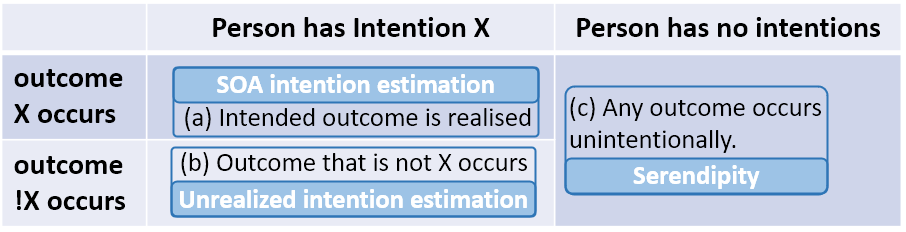
\includegraphics[width=\columnwidth]{samples/IntentQuad.png}
    \vspace{-5mm}
    \caption{Taxonomy of intentions: (a): realized intentions; (b): unrealized intentions; (c): serendipity}
    \vspace{-5mm}
    \label{fig:intent}
\end{figure}
An example of unrealized social intentions in-the-wild is best illustrated with Fig. \ref{fig:teaser} (d). We observe a conversing group containing participants A -- F at a professional networking event where F is speaking.  If we observe the gaze of E, we see that they are the only person not attending to F but is instead gazing at D. An observer might perceive this gaze to indicate an intention to talk to D. While state-of-the-art approaches would conclude that a system is successful in predicting E's intention if D and E start having a conversation, this is conceptually problematic. The perceived intention of E to speak to D is already observed irrespective of whether D and E finally converse.

\section{Challenges of Unrealized Intention Labelling In-the-Wild}
\label{sec:challenge}
In this paper, we take Bratman's \cite{bratman1987intention} definition of intentions by considering them as part of future action planning coupled with a belief by the individual that they have the ability to carry out the action. Crucially for intelligent systems, these planning behaviours need to be perceivable externally. 

Inherent challenges exist when framing intentions to be realizable or not. Pushing for technologies that work outside of the lab and in-the-wild adds even more difficulty. It relies more on training models to infer people's \emph{internal state}. Extracting this at high temporal fidelity and accurately is one bottleneck. The other is that there is no systematic approach to label unrealized intentions both in terms of the relevant cues and also the outcome that did not occur. 

The challenges of labelling intentions are illustrated in Fig. \ref{fig:selfvsthird}. For many, (including initially the authors themselves) self-report seems the only reasonable method to obtain labels of intentions. Ideally, the person would report constantly (\textbf{self-reported in-situ continuous feedback}: Fig. \ref{fig:selfvsthird}(a)), leading to a very temporally precise measure of someone's intention. Some tools have been developed to enable in-situ and in-the-wild reporting of affect whilst watching mobile video that may be applicable in this case \cite{zhang2020rcea}. However, this could disturb the spontaneity of the social behavior. Another alternative is to have subjects watch an interaction they just had and rate it continuously \cite{templeton2023long}. However this is hard to scale. Another solution involves individuals reporting their intentions just after finishing an interaction (\textbf{self-reported in-situ posthoc feedback}: Fig. \ref{fig:selfvsthird}(b)). However reflective cognitive processes can occur during post-hoc reflection leading to a difference in reported intention compared to a spontaneous in-situ report (see \cite{Dudzik2023} for a detailed discussion ). 
% Finally, whilst very powerful for artificial mind reading, self-report approaches for labelling intentions are hard to scale.
 
A final option uses external observers (\textbf{third-party continuous post-hoc feedback}: Fig. \ref{fig:selfvsthird} (c)). The temporal precision between the intention and sensor data is preserved, and the behaviour is not disturbed. However, whilst being much more scalable, it moves us further away from the truth of the individual being observed. There is perhaps still hope. By asking annotators to label plausible intentions, they are likely to simulate narratives plausible to their own life experiences \cite{Decety2004,emotions}. While this may not be the same as the true intention of the person, intelligent systems can still reason about these plausible perceptions, potentially updating and adjusting their understanding based on feedback during user interactions. Meanwhile the individual's true intentions are kept private. 
% other benefits including preserving the privacy of the subject until they want to reveal their true intention. However, in leveraging an annotator's own subjective life experiences, exploiting contextual knowledge from the setting will be important. However context estimation is another unsolved holy grail. 



\begin{figure}[tb]
    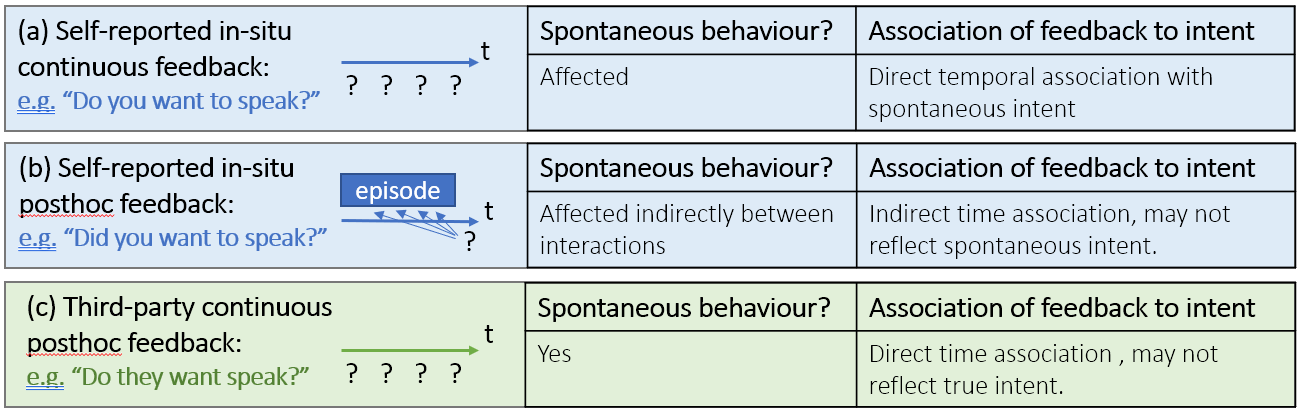
\includegraphics[width=\columnwidth]{samples/SelfvsThirdPartyIntentAnnotations_v3.png}
        \vspace{-5mm}
    \caption{Challenges to overcome for labelling realized and unrealized intentions. We present a study using (c) in Sec. \ref{sec:case}.}
        \vspace{-5mm}
    \label{fig:selfvsthird}
\end{figure}

% \begin{itemize}
%     \item why are unrealised intentions important to capture
%     \item what are we actually doing these days?
%     \item what make capturing unrealised intentions hard challenges of doing this in the wild (no standardised way of thinking about this, are realised and unrealise intentions observable in the same way? issues of semantics and resolution of that forces us to think more deeply about the truth we are searching for. 
% \item show that we cannot easily ask people whilst making it scalable
% still the issue of label sparsity as we may still miss quite a few observations. 
% \item Need datasets able to capture high quality audio as well as video so that we can characterise this. is this something that can be crowdsourced? 
% \item challenges of label noise, 
% \item need for some form of super annotator that is sensitive to these issues? Seeing things that no one else sees.
% A form of artificial empathy?
% \item First person or third party perceptions. ....The validity of truth.

% \end{itemize}
% Ethics of machines that can do it, ethics of machines that cannot do it?









% \noindent
% \subsubsection*{Main stream machine perception avoids cognitive modelling in machine perception tasks}
% % \vspace{-2mm}

% % Whilst there have been some great efforts to model intention in the HRI and HCI community, 

% \noindent
% Whilst this paper makes an argument for unrealized intention estimation, this particular usecase serves to highlight a major conceptual challenge we still face when injecting In other related mainstream computer science fields such as Computer Vision and Pattern Recognition, Su and Crandell highlight an important gap in the field observing that the community has shifted away from " [explaining] the internal cognition of people...[to] merely [describing] the external behavior of people" \cite{AffectiveGrowthCV2021}.




\section{Case Study: Estimating Unrealized Intentions to Speak} \label{sec:case}
As highlighted in Sec. \ref{sec:challenge}, there are compelling benefits to using third party labels. To this end, we present a case study that investigates two questions, focusing on the problem of speaking intention in-the-wild: (i) How feasible is it to label unrealized intentions using external observers? (ii) How could we train a model to detect realized and unrealized intentions? This section describes a case study to investigate this for estimating unrealized intentions to speak from the data shown in Figure \ref{fig:teaser} (b). This allows us to investigate how realized and unrealized intentions may be related and the challenges of doing this in a in-the-wild ecologically valid setting. 
% Second, we focus on the modality of body worn acceleration although the same setting could be extended to a multi-modal setup. 
\subsection{Related Work on Intentions to Speak}
To our knowledge, Wlodarczak and Heldner carried out the only research that has discussed unrealized intentions to speak \cite{wlodarczak2020breathing}. They used sensors strapped to the chest and abdomen in seated discussions to measure breathing during conversations. The findings identified breath inhalations (that looked like preparations to speak) followed by long breath holds and a silent exhalation with no accompanying speech activity. They speculated this behaviour could indicative of unrealized intentions. Their findings are foundational but their sensing approach is hard to scale to dynamic in-the-wild ecologically valid settings. 
% Moreover, their speculations were not validated with self-reports or continuous third-party perceptions of the multi-modal data. 

Other related work focused on behaviour forecasting, namely turn-change prediction and next-speaker prediction. 
% not in the wild
% Several studies have mentioned using multi-modalities 
% Several studies have found some related social cues and behavioral patterns of turn-changing in the conversations. The work of Petukhova and Brunt \cite{whosnext} found gaze aversions, lip movements and posture shifts are strongly correlated with receiving the next turn in conversations. According to Novick et al., 42\% of the turn changes follow the pattern: the speaker first looks towards the listener as they complete the turn; then the speaker and the listener have a short moment of eye contact; lastly the listener looks away and begins speaking \cite{novick_gaze}. Automatic recognition of such patterns can be useful for next speaker prediction and possibly for prediction of intentions to speak. In a multi-party conversation, turn-taking can also become rigid sometimes, as an interruption, which can be interpreted as ``not letting current speaker finish" \cite{schegloff2001accounts}.
Turn-change prediction estimates \emph{when} a turn change is about to occur whilst next-speaker prediction estimates \emph{who} will speak next. Petukhova and Bunt \cite{whosnext} found gaze aversions, lip movements, and posture shifts are strongly correlated with receiving the next turn in conversations. 
% According to Novick et al., 42\% of turn changes follow the pattern: the speaker first looks towards the listener as they complete the turn; then the speaker and the listener have a short moment of eye contact; lastly the listener looks away and begins speaking \cite{novick_gaze}. 
% As noted by Schegloff, turn-taking is not always smooth as an interruption could be interpreted as not letting the current speaker finish, which can be views conceptually as a form of unrealized intention \cite{schegloff2001accounts}.
 Gaze and respiration \cite{ishii2016prediction,ishii2015multimodal}, and mouth opening patterns \cite{mouth_open_patterns} are also commonly observed. 
% Ishii et al. showed that gaze-transition patterns are useful for predicting the next speaker and when the next speaker starts to speak . Later they found a fusion model using both respiration and gaze behaviour performs better than using only one of them, and respiration was the more useful feature in their multimodal model \cite{ishii2015multimodal}. A followup study also by Ishii et al. found people tend to open their mouths slightly before they start speaking, which can be related to intentions to speak \cite{mouth_open_patterns}. 

% Turn-taking related features have also been used to predict the next speaker in a conversation. 

% Malik et al. \cite{malik2020speaks} found that pause duration and addressee role were also important cues. 

% Ishii et al. \cite{ishii2016prediction} showed that gaze-transition patterns are useful for predicting the turn-changing or turn-keeping, the next speaker in turn-changing, and the timing of the start of the next speaker's utterance.
% Importantly, respiration was found to be the more useful feature in their multimodal fusion model.
% This could not only be a turn-initial signal, but also related to intentions to speak \cite{mouth_open_patterns}. 
% Many studies related to next speaker prediction have mentioned the importance of combining multi-modalities provide better and more robust performance \cite{ishii2015multimodal} \cite{mouth_open_patterns} \cite{respiration_with_sensors}. 

% Combining multi behavioral features includes more social cues of start speaking than single modality. 

\subsection{Our Approach} 
\begin{figure}[bt]
  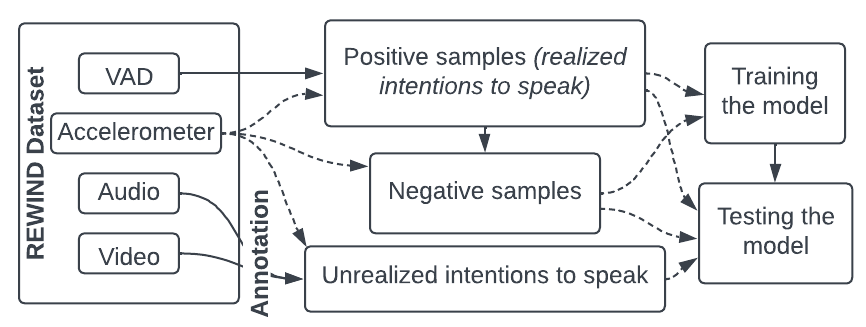
\includegraphics[width=0.45\textwidth]{samples/INTS_overview (6).png}
  \vspace{-5mm}
  \caption{Overview of our approach. The dashed lines indicate the flow of only accelerometer data. 
% Note that the model is \emph{not} trained on the unrealized intentions to speak.
}  \vspace{-6mm}

  \label{fig:overview}
\end{figure}
% Using (heuristically) smoothed VAD, successful cases (windows) of intentions to speak are automatically extracted. These are used as positive samples for the model.
% Randomly selected windows without overlap with successful cases are extracted and used as negative samples for the model.

Since we argue for the development of systems that work out of the lab in in-the-wild ecologically valid settings, we wanted to investigate the efficacy of exploiting a sensing setup that would maximise the detection of unrealized intentions and privacy. Building on the promising results of estimating speaking status with accelerometers \cite{raman2022conflab,rewinddata} we leverage the ubiquity of the conference ID badge commonly hung around the neck. The badge form-factor can be exploited with sensors such as a tri-axial accelerometer which is most likely to capture the fine grained breathing activities observed by Wlodarczak and Heldner \cite{wlodarczak2020breathing}, as well as other intention related behavioural modalities (e.g. leaning, gaze via head pose). 
% Given that the chatter of the social event is quite loud, participants may also tend to speak a bit louder, leading to possibly more exaggerated breath inhalations. 
Given the loud background chatter, we decided against using the audio since detecting subtle noises could be more challenging. Moreover, there are privacy concerns when recording private conversations \cite{raman2022conflab,MnM2021_underline}. Multi-modal analyses are left for future work. 
% 
% We aim to infer perceivable intentions to speak in a privacy-preserving and ubiquitous way. Since accelerometers capture a superposition of useful behavioural modalities for intentions to speak, we do this inference based on accelerometer data only. Examples of such features are body movement, posture shifts, possibly breath patterns. This final feature will likely not be captured in fine-grained detail, as a wearable accelerometer such as a smart badge will not be as sensitive as a specialized breath sensor. This is a trade-off because specialized breath sensors are not feasible in-the-wild. 
% Towards this goal of inferring intentions to speak, 

Our experimental approach is summarized in Fig. \ref{fig:overview}; a model is trained on the accelerometer data of automatically extracted \emph{realized} intentions to speak (Sec. \ref{sec:training}), the trained model is evaluated on automatically generated realized and also manually annotated unrealized intentions to speak (Sec.\ref{sec:annot}), as discussed in Sec. \ref{sec:res}.
% A classifier is trained on the accelerometer data of realized intentions to speak (as positive samples) and randomly selected negative samples, such that there is no overlap with the positive samples. These positive samples are automatically extracted from the voice activity detection (VAD) as explained in section \ref{sec:vad}. The trained classification model is then evaluated on annotated cases of unrealized intentions to speak. These annotated cases are only used for evaluation and not for training due to the small amount of annotated cases. An overview of our method is shown in Figure \ref{fig:overview}.




% \begin{figure*}
%   \begin{tabular}{cc}
%      \begin{tabular}{l} 
%         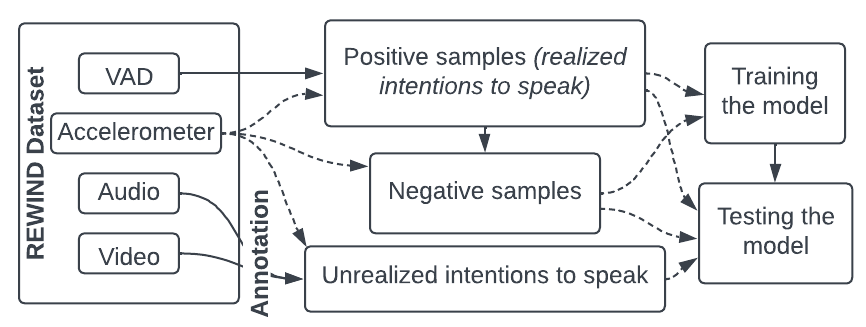
\includegraphics[width=0.48\textwidth]{samples/INTS_overview (6).png} 
%      \end{tabular}& 
%      \begin{tabular}{l} 
%         \includegraphics[width=0.4\textwidth]{samples/vad4.jpg}\\
%      \end{tabular}
%   \end{tabular}
%   \caption{\emph{Left:} A graphical overview of the case study; a model is trained on the accelerometer data of automatically extracted realized intentions to speak. This model is evaluated on annotated unrealized intentions to speak. Dashed lines indicate the flow of only accelerometer data. Note that the model is \emph{not} trained on the unrealized intentions to speak. \emph{Right:} Visualization of the VAD processing; short pauses are smoothed, short turns are ignored and a window of length \emph{x} before speech is used as a positive sample. The top image represents the raw voice activation. The bottom image represents the corresponding processed VAD.}
%   \label{fig:overview_and_vad}
% \end{figure*}



% \subsection{Exploratory Study of unrealised Intentions to Speak [merge with next]}
% \textbf{[Sketch: JORD]}
% Tried to become self-aware of cues that we think (can) indicate intentions to speak + dug in literature for cues, and listed all these cues
% => first word/syllable of utterance
% => hand raise
% => gaze patterns
% => deep breath to start speaking
% => mouth patterns (1. as proxy for breath patterns, 2. bite/compress/lick lip)
% => posture shifts
% => indirect; (attempt at) refusal to yield turn (talk louder / more fillers)
% => general body movement / motion distribution (Hayley had a nice graph for this)

% Looked at the REWIND dataset, looking for cues that (might) indicate an intention to speak
% => differentiate intentions to start speaking and intentions to continue speaking
% => audible mouth-opening patterns (lip/tongue click/smack)
% => lean towards other peoples ear in the presence of outside noise (essentially a posture shift, but a specific one)
% => throat clears

% We have a hunch that humans unconsiously are very good at inferring intentions to speak (e.g. based on gaze behaviour). Tried to explicitly look for them in private/personal social situations (drink with friends). => audible mouth-opening patterns (e.g. person A has an intention to speak, opens their mouth and by doing so smacks their lips. Then everybody looks at A expecting them to start speaking, and then A starts speaking) 

\subsection{Experimental Data}
We use the REWIND dataset \cite{laughterquiros2023} (obtained via personal communication with the authors) which will soon be shared \cite{rewinddata}. The REWIND dataset contains audio, video, and wearable accelerometer data of an indoor professional networking event with around 100 attendees who stood and were free to mingle as they pleased. Video data is recorded by elevated side-view cameras, as shown in Fig. \ref{fig:teaser} (c). The event offered a mixed consent model where participants could choose whether to wear an accelerometer around their neck (like a conference ID badge), a wireless microphone attached to the face via specialised tape used for theatre productions, and appear under the cameras. A 10-minute segment (1:00:00 - 1:10:00) of the data is used for the exploratory study and annotations. In this interval, 13 participants had audio, video, and accelerometer data. Ethical approval from the university ethics board was granted.


\subsection{Labelling Unrealized Intentions to Speak}
\label{sec:annot}
To assess the quality of the model on unrealized intentions to speak, a sample of unrealized intentions to speak is needed. Before labelling the data, an initial exploratory study of unrealized intentions to speak was done. This involved critically examining our own behaviour in cases of intentions to speak and that of others. Finally, the data was observed to find cues that indicate intentions to speak. 

From this observation, we found an important conceptual distinction between intentions to start speaking and intentions to continue speaking. Another important finding was that mouth-opening patterns through lip or tongue smacks were audible in some cases. Due to the loud background chatter, we found that people sometimes lean in or shift posture towards someone's ear when they want to say something. Lastly, throat clearing seemed also to indicate an intention to speak.

% After the exploratory study, samples of unrealized intentions to speak are generated by annotating a 10-minute segment (1:00:00 - 1:10:00) of the data. In this interval, 13 participants who had audio, video, and accelerometer data.
% were annotated A segment of 10 minutes was chosen because more would not be feasible given the time and resource limitations of this project, and this 10-minute window would need to be multiplied by the number of relevant participants (13, after removing the participants not in view of any camera) in order to get the total annotated time. 
% The segment was chosen to be 1:00:00 until 1:10:00 where participants were mingling. 
% This is somewhat arbitrary, but it does fulfil the requirement that the participants can move freely and talk to whom they want and about any topic they desire (e.g. the participants are not collectively listening to a public speaker and are not asked to play a conversational game with assigned conversation partners). 
% Taking the intersection of participants with a microphone and an accelerometer, and removing participants that are not in view of any camera in the segment, and with fully working audio date, 13 relevant participants remain. 
% There was one person with audio issues, so in the end there were 13 participants of interest.

% Given this segment, one (native Dutch) of the authors of this work performed the annotation 
After the exploratory study, during the 10-minute segment, start and end times of perceived unrealized intentions to speak were labelled manually. Annotations were performed by one of the co-authors
using ELAN \cite{elan} using audio-visual data coming from the microphone and corresponding camera of a given subject. 
% The annotator listened to one participant at a time while looking at them through the camera in which they are best visible. 
% When the annotator perceived a (likely) unrealized intention to speak, this segment was annotated. This is primarily based on human intuition.
% Given the subtle nature of the task, the annotations can be subjective. 
Following the findings of the exploratory study, we identified two categories of unrealized intentions. We report the number of observed unique individuals, samples, and mean and standard deviation of the interval lengths respectively: intentions to take the turn (\textbf{UnrealStart}: $10,22,1.98\pm0.89s$ ) and intentions to continue speaking (\textbf{UnrealCont}: $7,17,2.46\pm0.97s$). 
% After the annotations were finished, they were processed to a usable format in Python using the pympi library \cite{pympi-1.70} and will be shared.



\subsection{Training Intentions to Speak}
\label{sec:training}
% To scrutinize the potential utility of an accelerometer for detecting speech intention, 
Four distinct models were trained with varying window lengths spanning 1s-4s with 10 epochs under 3-fold cross-validation. To minimise variation in the model performance to discern differences between the different experiments, Leave-person-out cross validation was not used. With so few test samples, we decided to train models for just \emph{realized} intentions to speak and test on the samples identified in Sec. \ref{sec:annot}. These models were evaluated using the ROC AUC across 5 experiments using different types of positive test samples \footnote{code and data shared at \url{https://github.com/llt-warlock/unrealizedIntention}}; \textbf{1. All}: realized and unrealized intentions, \textbf{2. Realized}, \textbf{3. Unrealized}, \textbf{4. UnrealStart}: unrealized intentions to start speaking, and \textbf{5. UnrealCont}: unrealized intentions to continue speaking. Adapting the implementation of Vargas et al. \cite{laughterquiros2023}, the structural architecture of our models comprises multiple residual neural networks embedded within convolutional neural networks. Non-overlapping training samples from individual accelerometer data were sampled from the mingling time outside of our chosen 10 minute segment and within the 10 minute segment for the test data.  This procedure was repeated 100 times. 

\subsubsection{Voice Activity Pre-processing}
\label{sec:vad}
For each speaker, we process the provided automatically detected voice activity generated by REWIND which computes voice activity by applying the following to each audio signal; loudness normalization, denoising, and Speaker diarization via NVIDIA NeMo \cite{kuchaiev2019nemo}. This was then processed to remove extremely short turns (1.5s) that are likely to be back-channels and short pauses (1.5s) between speaking. The threshold was determined empirically. 
% address two specific challenges. The first challenge pertains to microphone activation caused by short backchannels, while the second challenge involves microphone deactivation when a speaker momentarily pauses but maintains the turn. These issues are effectively resolved through preprocessing techniques. 
% In the Voice Activation Files (VAD) methodology, pauses shorter than 1.5 seconds are assigned a value of 1, indicating activation. Similarly, turns shorter than 1.5 seconds are assigned a value of 0, indicating deactivation. 
% It is important to note that these numerical thresholds have been optimized through a manual empirical process. 
% The smoothing procedure is illustrated in the left part of of Fig. \ref{fig:vad}. 

% \begin{figure}[tb]
%   \includegraphics[width=0.35\textwidth]{samples/vad5.jpg}
%   \vspace{-5mm}
%   \caption{Visualization of a smoothed voice activity signal; see Sec. \ref{sec:vad} for details. All positive samples are located just before the onset of speech (red) with duration \emph{x}. y axis: presence(1) or absence (0) of voice activity. }
%     \vspace{-5mm}
%   \label{fig:vad}
% \end{figure}



% \begin{figure}[hb]
%   \includegraphics[width=0.5\textwidth]{samples/vad2.jpg}
%   \caption{Visualization of the VAD processing; pauses are smoothed, short turns are ignored and a window of length \emph{x} before speech is used as a positive sample.}
%   \label{fig:vad}
% \end{figure}

% \begin{figure}[hb]
%   \includegraphics[width=0.43\textwidth]{samples/vad4.jpg}
%   \caption{Visualization of the VAD processing; short pauses are smoothed, short turns are ignored and a window of length \emph{x} before speech is used as a positive sample. The top image represents the raw voice activation. The bottom image represents the corresponding processed VAD.}
%   \label{fig:vad}
% \end{figure}

\subsubsection{Positive Sample Set Generation}
The positive realized intention samples were selected as the time windows prior to the activation of voice activity (interval X in Fig.\ref{fig:vad}). As the time window increases, the number of positive samples decrease due to a higher chance of overlapping with speaking segments. The length of time for the annotated unrealized intention positive samples varies (as mentioned in Sec. \ref{sec:annot}). Since there were so few samples, we decided to use them all irrespective of the window length. In all experiments, we aligned the end of the sample with the annotated end time of the positive unrealized intention sample and then computed back in time for the corresponding window length. As the time window increases, there may be more frames of speaking. The number of positive samples for training and test are shown in Tab. \ref{tab:experiment}.
% : the number of positive samples of "realized intention" varies under different time windows, while the number of positive samples of "unrealized intention" remains the same.  
\begin{figure}[tb]
  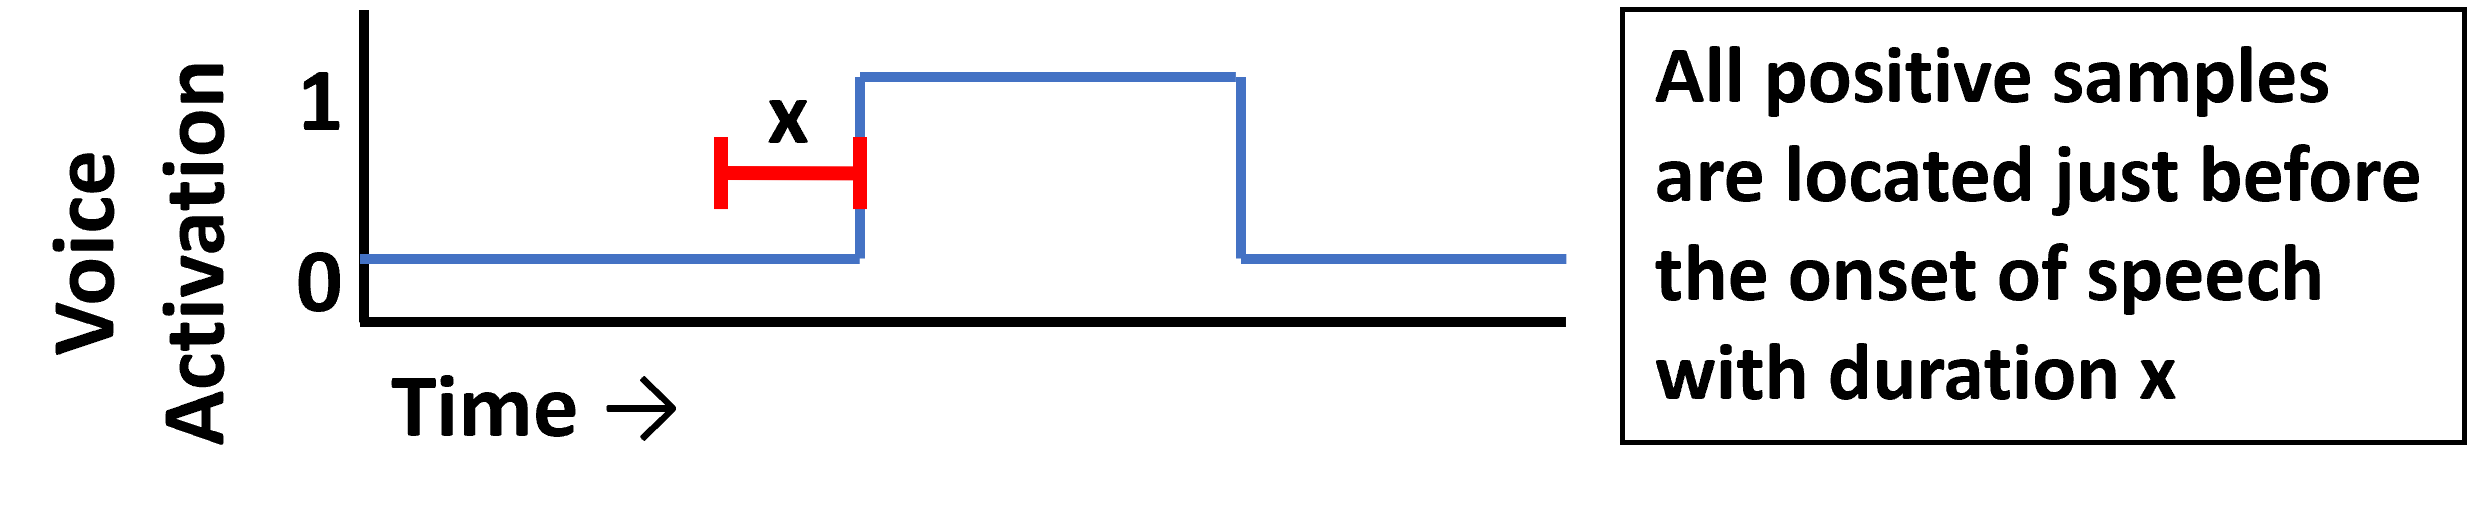
\includegraphics[width=0.43\textwidth]{samples/vad10.png}
  \vspace{-4mm}
  \caption{Positive sample generation; X is varied from 1-4s.}
    \vspace{-2mm}
  \label{fig:vad}
\end{figure}




% \begin{table}[H]
% \centering
% \scalebox{0.7}{
% \begin{tabular}{|l|c|c|c|c|}
% \hline
% \textbf{Experiment} & \textbf{\makecell[c]{realized \\ intention}} & \textbf{\makecell[c]{unrealized \\ intention (start)}} & \textbf{\makecell[c]{unrealized \\ intention \\ (continue)}} & \textbf{\makecell[c]{number of \\ positive \\ samples}} \\ \hline
% \textbf{Training} & $\checkmark$ &  & & 2894 \\  \hline
% \textbf{All} & $\checkmark$ & $\checkmark$  & $\checkmark$ & 327 \\  \hline
% \textbf{Realized}  & $\checkmark$  &  &  & 286\\ \hline
% \textbf{Unrealized}  &   & $\checkmark$ & $\checkmark$  & 41 \\ \hline
% \textbf{UnrealStart}  &   & $\checkmark$ &  & 22 \\ \hline
% \textbf{UnrealCont}  &   &  & $\checkmark$  & 19 \\ \hline

% \end{tabular}
% }
% \caption{Test dataset of experiments}
% \label{tab:experiment}
% \end{table}

\begin{table}[b!]
  \centering
  % \scalebox{0.4}
  
  \begin{tabular}{|c|c|c|c|c|} \hline 
      \multicolumn{2}{|c|}{} & \textbf{Realized}& \textbf{\makecell[c]{Unrealized\\Start}}&\textbf{\makecell[c]{Unrealized\\Continue}} \\ \hline

    \multicolumn{2}{|c|}{Train} & \cellcolor{cyan!15}2567 / 2053 / 1689 / 1487 &\cellcolor{red!5} unused &\cellcolor{red!5} unused \\ \hline

  { \parbox[t]{2mm}{\multirow{5}{*}{\rotatebox[origin=c]{90}{Test}}}}  & 1 &\multicolumn{3}{c|}{\cellcolor{cyan!15}327 / 268 / 239 / 217 }  \\ \cline{2-5}
    &2 & \cellcolor{cyan!15}286 / 227 / 198 / 176 &\cellcolor{red!5}unused &\cellcolor{red!5} unused  \\ \cline{2-5}
    &3 & \cellcolor{red!5} unused &  \multicolumn{2}{c|}{\cellcolor{cyan!15}39/39/39/39}   \\ \cline{2-5}
    &4 & \cellcolor{red!5} unused & \cellcolor{cyan!15}22/22/22/22 & \cellcolor{red!5} unused \\ \cline{2-5}
    &5 & \cellcolor{red!5} unused  & \cellcolor{red!5} unused & \cellcolor{cyan!15}17/17/17/17    \\ \hline
  \end{tabular}
  \caption{Numbers of positive samples by type: row 1. training; row 2-6: test samples generated at 1s/2s/3s/4s window lengths.}
  \vspace{-5mm}
  \label{tab:experiment}
\end{table}



\subsubsection{Negative Sample Set Generation}
\label{negative sample set}
% In addition to the predetermined positive samples of accelerometer data, which are accompanied by a time window interval immediately preceding the speaking state, the 
Negative samples of length 1s-4s depending on corresponding experiment length. Trainig samples were randomly sampled outside the period 1:00:00-1:10:00. Test samples were taken during the time interval of 1:00:00-1:10:00 taking care that they did not overlap with any of the positive samples (expt. 2). Test samples for experiments 3-5 were randomly generated and did not overlap with positive realized or unrealized intention samples. The negative samples generated for experiment 1 also included the negative samples of experiments 2 and 3. The ratio of positive to negative samples is always 1:20.

% the negative samples randomly sampled in Experiment 2 did not overlap with the time periods of the positive samples of realized intentions. The negative of experiments 3, 4, and 5 samples were randomly generated and did not overlap with the time period of corresponding positive samples (Table \ref{tab:experiment}) and realized intention samples. The negative samples generated in Experiment 1 were a combination of the negative samples from Experiments 2 and 3. The ratio of positive samples to negative samples is maintained at 1:20. 

\subsection{Results}
\label{sec:res}
% \subsubsection{Evaluation of the model}
% For all experiments, the trained models were used to analyze the classification quality on the test sets under four different time windows. This procedure was repeated 100 times
% to make the results more stable and 
% to get a reliable estimate of the means and standard deviations of the AUC. 
Results compared are shown in Fig. \ref{fig:all-result} where the mean and standard error were computed over all folds over 100 runs. We observe that \textbf{Realized} had above average performance with better performance for longer windows and that \textbf{All} performs worse but still mostly above average. \textbf{Unrealized} shows performance comparable to \textbf{Realized} for 1s and 2s windows. However \textbf{Unrealized} has poor performance at windows of 3s or 4s. Finally, dividing the data from \textbf{Unrealized} up, \textbf{UnrealCont} has consistently worse performance while \textbf{UnrealStart} has better performance than all other experiments for 1s and 2s windows. This suggests that Unrealized intentions to start speaking exhibit extremely clear non-verbal behaviors where the good performing time window lengths are commensurate with the observation of leaning. We speculate that unrealized intentions to continue speaking have more subtle behaviour since the subjects did not need to coordinate a turn change. The comparable performance of \textbf{UnrealCont} at 1s suggests that distinguishing behaviours are short such as for breathing. Finally The general decreasing trend of experiments 3-5 as the window size increases may be due to samples being more and more contaminated by voice activity behavior. 
% This provides evidence that intention to speak behavior is very different from speaking behaviour.



% According to the results, the models trained with 1s and 2s windows can identify some patterns of unrealized intentions to speak but perform worse as the window size increases. Since we kept all the samples as the window length grew, we speculate that this could be related to the test window being increasingly contaminated with moments of voice activity. 
% For unrealized intentions, the models perform better with a shorter time window size. Due to the method of how we generated positive samples for unrealized intentions, as the size of time window increased, these samples would contain invalid data, which might reduce the performance. We speculate that unrealized intentions tend to happen in a small period of time, increasing the time window size can include less informative data related to unrealized intentions. 

% For unrealized intentions, the mean AUC decreases as the time window increases. For the realized intentions, the mean AUC score first decreases before the 2-second window, and then increases and reaches to the highest of all the five experiments after 2 seconds. In the first two windows, the model performs the best at predicting the unrealized intentions to start speaking. 

\begin{figure}[tb]
  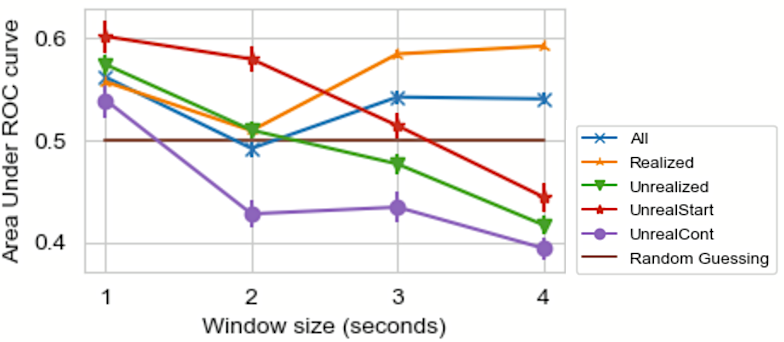
\includegraphics[width=0.5\textwidth]{samples/result-all-2.png}
  \vspace{-5mm}
  \caption{ 
  Mean and standard deviation for all experiments.
}
\vspace{-5mm}
  \label{fig:all-result}
\end{figure}


% \begin{table}[H]
% \centering
% \scalebox{0.7}{
% \begin{tabular}{|l|l|l|l|l|}
% \hline
% \textbf{AUC scores}  &  \textbf{1 second}  & \textbf{2 seconds} & \textbf{3 seconds} & \textbf{4 seconds} \\ \hline
% \textbf{all intentions to speak} & 0.5618 (0.007)  & 0.4919 (0.008) & 0.5423 (0.007) & 0.5405 (0.006)\\ \hline
% \textbf{realized}  & 0.5573 (0.004) & 0.5093 (0.004)  & 0.5846 (0.004)  & 0.5923 (0.004) \\ \hline
% \textbf{unrealized} & 0.5742 (0.010) & 0.5098 (0.009) & 0.4766 (0.010) & 0.4168 (0.009)\\ \hline
% \textbf{unrealized (start)} & 0.6018 (0.016) & 0.5796(0.012) & 0.5142 (0.012) & 0.4442 (0.014) \\ \hline
% \textbf{unrealized (continue)} & 0.5393 (0.018) & 0.4276 (0.013) & 0.4342 (0.015) & 0.3939 (0.011)\\ \hline

% \end{tabular}
% }
% \caption{Mean (standard deviation) of ROC AUC scores for the evaluation on realized intentions to speak, unrealized intentions to start speaking and unrealized intentions to continue speaking.}
% \label{tab:auc_results}
% \end{table}


% \subsubsection{Comparison to random guessing}
% To compare the model's performance to random guessing, t-tests were done. The null hypothesis is $H_0$: ``The model performs the same as or worse than random guessing". The alternative hypothesis is $H_1$: ``The model performs better than random guessing". For each model evaluation configuration, as in table \ref{tab:auc_results}, a mean and a standard deviation of the AUC scores exist. Random guessing has a mean AUC of 0.5. In addition, we assume that the standard deviations of the AUC for random guessing are the same as the standard deviations in table \ref{tab:auc_results}. One-sided t-tests are done to see if the model performs better than random guessing. The p-values of the t-tests are given in table \ref{tab:ttest}. The values are compared to the (conservative) threshold of 0.001. 

% the comparison results are indicated with color in the table. Green color means that the result is significant and the null hypothesis can be rejected, meaning that the model performed better than random guessing. Red color means that there is not enough evidence to reject the null hypothesis.

% \begin{table}[h]
% \centering
% \scalebox{0.7}{
% \begin{tabular}{|l|l|l|l|l|}
% \hline
% \textbf{p-values}  & \textbf{1 second}  & \textbf{2 seconds} & \textbf{3 seconds} & \textbf{4 seconds} \\ \hline
% \textbf{all intentions to speak} & 6.545e-185 & 4.287e-138 & 1.0000 & 1.0000\\ \hline
% \textbf{realized}  & 4.889e-77 & 1.099e-29  & 0.2402  & 0.9996 \\ \hline
% \textbf{unrealized} & 1.575e-88 & 1.166e-98 & 1.0000 & 1.0000\\ \hline
% \textbf{unrealized (start)} & 3.130e-33 & 3.069e-138 & 1.293e-53 & 1.725e-125 \\ \hline
% \textbf{unrealized (continue)} & 1.241e-115 & 5.528e-75 & 0.9974 & 1.0000\\ \hline
% \end{tabular}
% }
% \caption{P-values for the t-tests comparing the model performance to random guessing. }
% \label{tab:ttest}
% \end{table}

% \begin{table}[h]
% \centering
% \scalebox{0.7}{
% \begin{tabular}{|l|l|l|l|l|}
% \hline
% \textbf{p-values}  & \textbf{1 second}  & \textbf{2 seconds} & \textbf{3 seconds} & \textbf{4 seconds} \\ \hline
% \textbf{all intentions to speak} & 2.099E-96 & 1.000 & 5.868E-82 & 6.081E-86\\ \hline
% \textbf{realized}  & 1.508E-144 & 8.249E-38  & 4.206E-135  & 2.894E-135 \\ \hline
% \textbf{unrealized} & 3.244E-90 & 6.793E-19 & 1.000 & 1.000\\ \hline
% \textbf{unrealized (start)} & 1.082E-82 & 6.732E-83 & 6.923E-20 & 1.000 \\ \hline
% \textbf{unrealized (continue)} & 4.442E-40 & 1.000 & 1.000 & 1.000\\ \hline
% \end{tabular}
% }
% \caption{P-values for the t-tests comparing the model performance to random guessing. }
% \label{tab:ttest}
% \end{table}


% \subsubsection{Linear regression through AUC scores}
% To explore the trends of increasing the size of the time window statistically, linear regression is applied. The slopes found by linear regression through the results of each experiment are presented in Table \ref{tab:regress}. Additionally, the $R^2$ measure (coefficient of determination) is presented. This measure indicates how well the regression model fits the data.

% \begin{table}[h]
% \centering
% \scalebox{0.7}{
% \begin{tabular}{|l|l|l|}
% \hline
%                         & \textbf{Slope} & \textbf{$R^2$} \\ \hline
% \textbf{All intentions to speak} & -0.0281 & 0.927 \\ \hline
% \textbf{Successful}              & -0.0253 & 0.750 \\ \hline
% \textbf{Unsuccessful}            & -0.0309 & 0.711 \\ \hline
% \textbf{Unsuccessful (Start)}    & 0.0063 & 0.0658\\ \hline
% \textbf{Unsuccessful (Continue)} & -0.0473 & 0.967 \\ \hline
% \end{tabular}
% }
% \caption{Slopes and $R^2$ values for linear regressions through the results. $R^2$ close to 0 indicates a bad fit and close to 1 indicates a good fit.}
% \label{tab:regress}
% \end{table}

% \subsubsection{Difference between intention to start and continue speaking}
% For every window size, a Welch's t-test\footnote{Does not necessarily assume equal variance for the two samples.} is performed, comparing the data. The null hypothesis is $H_0$: ``The samples have the same mean". The alternative hypothesis is $H_1$: ``The samples have different means".
% The p-values for a window size of 1, 2, 3, and 4 seconds are 1.979e-89, 4.843e-93, 5.594e-62, and 3.325e-175 respectively. Hence, for each considered window size, the null hypothesis can be rejected. 


\section{Conclusion and Discussion}
%unrealized intentions CAN be perceived and can be detected. But the semantic gap is larger. This leads to the issue of subjectivity.
%how often do unrealized intentions occur? How would learned representations handle these types of behaviors? What is the common pattern when unrealized intentions occur? probably the outcome constellation looks very different... or perhaps too varied to learn any regular patterns from?
%
We have proposed a reframing of intention estimation research to account for both realized and unrealized intentions to overcome the "intention by outcome" problem. We carried out a preliminary investigation showing that unrealized intentions can be labelled by an external observer. Our experiments using trained models demonstrate that realized and unrealized intentions are hard to disentangle which suggests potential opportunities to exploit transfer learning approaches. Beside this, many open questions remain:

\paragraph{Subjectivity}
Our case study used one annotator. Without an associated outcome, unrealized intention labelling requires an observer to fill the gap between the observed cues and the perceived intent using on their own life experiences. Usually subjectivity is treated as noise but is there not a validity to any perception as long it is explained by observed cues? If so, how can we train models to account for this? This could allow systems to be designed to take only certain types of biases into model training based on a careful selection of the context of annotators.
As argued by Dudzik et al., a lack of systematic treatment of annotator context could be limiting system performance for affect perceptions\cite{dudzik2019context} and could apply to other labelling tasks. 

\paragraph{Localizing Intentions and Time} Temporal granularity was lost with our detection based model. Our experiments shows no consistent trend across the different window sizes. Using localization methods may improve performance. Labelling the end time for unrealized intentions needs further investigation ; how long should a system wait before declaring an intention to be (un)realized? 

\paragraph{Longer-term Intention Estimation}
The case study focused on a relatively short term intention. How does the problem change if more complex intentions are considered? e.g. intentions to join, leave a conversation, or start a conversation.

\paragraph{Multimodality}
Labelling the unrealized intentions required multimodal stimuli, although audio was the primary modality used. Multi-modal approaches worked well with realized intention estimation should be investigated for unrealized intent. 

\paragraph{Relating True with Externally Perceived Intention}
While there are scaling benefits to the third-party observer approach, we cannot deny the importance of the true intent of a user. There may be opportunities here to exploit third-party labels for personalization.

\paragraph{Potential for Societal Benefit} 
How should a system respond to and act upon automated perceptions of realized and unrealized intentions? The matter may need to be handled extremely carefully for applications that counter discrimination and exclusion, especially when making an incorrect inference could be extremely damaging. However the potential benefits are yet to be explored.


%%
%% The acknowledgments section is defined using the "acks" environment
%% (and NOT an unnumbered section). This ensures the proper
%% identification of the section in the article metadata, and the
%% consistent spelling of the heading.
% \begin{acks}
%Thanks to Tiffany, Stephanie, and Catha for their helpful feedback. 
% \end{acks}

%%
%% The next two lines define the bibliography style to be used, and
%% the bibliography file.
\pagebreak
\bibliographystyle{ACM-Reference-Format}
\bibliography{samples/references}


%%
%% If your work has an appendix, this is the place to put it.
% \appendix

% \section{Research Methods}

% \subsection{Part One}



\end{document}
\endinput
%%
%% End of file `sample-sigconf.tex'.
